
\chapter{Radiosity Problem formulation and Integral Equation}

In this section we formulate radiosity problem and corresponding radiosity integral equation. After defining the problem possible solution methods has been discussed at the end of the section.
\section{Problem definition}
The radiosity problem is special case of more general problem of global illumination. In other words radiosity is global illumination problem with scene composed of only lambertian surfaces. With this assumption of lambertian surfaces we now define the problem mathematically.
Radiosity $B(x_1,y_1)$ at point is power per unit area that leaves a point $(x_1,y_1)$ on a surface. The problem is to find the radiosity function over domain of all the surfaces in the scene given the following data,
1. $E(x_1,y_1)$, radiosity of emitters(light source) of scene
2. $K(x_1,y_1,x_2,y_2)$, ratio of radiosity received by point $(x_1,y_1)$ to radiosity radiated by point $(x_2,y_2)$  which can be calculated given the geometric location of the surfaces. 
3. $p(x_1,y_1)$ reflectivity of the surface at point $(x_1,y_1)$
Where, $(x_2,y_2)$  {\bf belongs to} domain of all the surfaces of the scene.
\section {Radiosity Integral Equation}
Radiosity is governed by an non-homogeneous Fredholm integral equation of second type which arise form more general problem of heat transfer known as rendering equation[Kajia]. The equation is shown in eq. (\ref{eq:3drie}). The radiosity $B(x_1,y_1)$ at point $(x_1,y_1)$  is sum of emitted radiosity and reflected radiosity received from all the points $(x_2,y_2) \in M^2$,  domain of all the surfaces in the scene.\\
{\bf show equation (1)}\\

{\bf show general fredholms equation}\\

\begin{equation} \label{eq:3drie}
B(x_1,y_1)=E(x_1,y_1)+p(x_1,y_1)\int_{M^2}K(x_1,y_1,x_2,y_2)B(x_2,y_2)dx_2dy_2
\end{equation}
In eq. (\ref{eq:3drie}) the integral is over all the points in domain of all  the surfaces $M^2$ in the scene. 

The kernel $K(x_1,y_1,x_2,y_2)$ is calculated from geometric location of the surfaces and can be expanded as shown in the eq. (\ref{eq:3dkernel}) which consist of cosine of angle made by local surface normals with a vector connecting two points, the distance  $r_{12}^{-d}$ between the two points (see Figure 1) and the visibility function which takes values from \{0,1\}. The constant c accounts for normalization of the integration. \\
{\bf need to see this as eq. (\ref{eq:3dkernel}) is explained as general kernel}\\
{\bf show equation (2)}\\
\begin{equation} \label{eq:3dkernel}
K(x_1,y_1,x_2,y_2) = c \cos \theta_1 \cos \theta_2 r_{12}^{-d} V(x_1,y_1,x_2,y_2) \\ 
\end{equation}
{\bf show Figure (1)}\\
\begin{figure}[h]
\centering
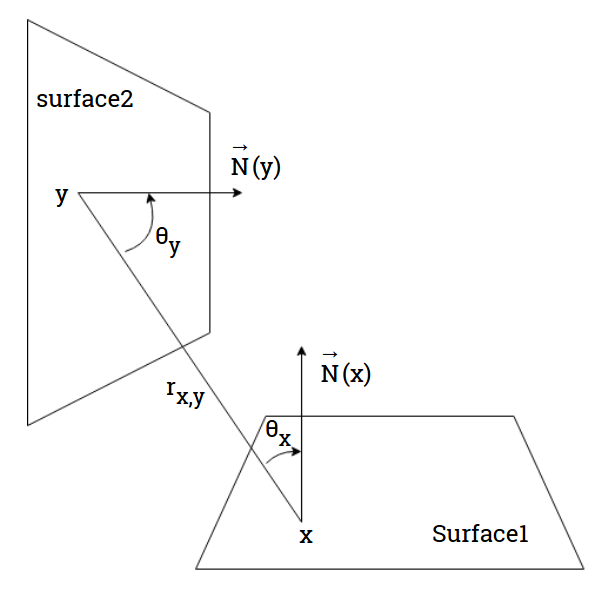
\includegraphics[width=0.4\linewidth]{xy.png}
\caption{This image will be referenced below}
\label{fig:xytheta}
\end{figure}\\
The parameters c and d takes value depending on  the scene. For 2D scenes, a scene consisting of lines instead of surfaces, d takes the value 1 and c takes the value 1/2 and the domain of the points is 1D. In the case of 3D scenes d takes the value 2 and c takes the value 1/$\pi$. From this point onwards we will refer to points by x and depending on the context (1D or  2D) it will be defined. The eq. (\ref{eq:3drie}) can be written as shown in eq. (\ref{eq:genrie})\\\\
{\bf show equation (3)}
\begin{equation} \label{eq:genrie}
B(x)=E(x)+P(x)\int K(x,y)B(y)dy\\\\
\end{equation}
\section{Analytical Solution}
In literature lot of methods where developed to solve the non-homogeneous Fredholm integral of second kind[ie survey][other ref]. In particular, if the kernel K is degenerate one can find exact solution of the radiosity integral equation[ie survey]. But for even simple 2D scene the kernel is non degenerate. If analytical solution is not possible then one can solve the problem by approximation methods like Collocation Method, Galerkin Method etc. {\bf But the size of the radiosity problem makes it difficult to use this methods}. We therefor use finite element methods(FEM) to compute approximate solution. We write unknown radiosity function as linear combination of basis function. Thus the problem get casted to system of linear equations which can be solved and approximate solution can be computed.In other words we solve the problem in finite dimensional space(domain). This method is also known as projection methods. More on this is discussed in next section.

